\documentclass{stdlocal}
\begin{document}
\section{Quad-Edge Algebra} % (fold)
\label{sec:quad_edge_algebra}

\begin{figure}
  \centering
  \begin{subfigure}[b]{0.4\linewidth}
    \centering
    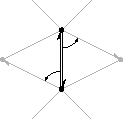
\includegraphics[width=\linewidth]{figures/quad-edge-edge.pdf}
  \end{subfigure}
  \hfill
  \begin{subfigure}[b]{0.4\linewidth}
    \centering
    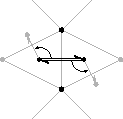
\includegraphics[width=\linewidth]{figures/quad-edge-dual.pdf}
  \end{subfigure}
  \caption[Quad-Edge Scheme]{
    \textbf{Quad-Edge Scheme}\\
  }
\end{figure}

\begin{figure}
  \centering
  \begin{subfigure}[b]{0.31\linewidth}
    \centering
    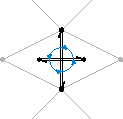
\includegraphics[width=\linewidth]{figures/quad-edge-rot.pdf}
  \end{subfigure}
  \hfill
  \begin{subfigure}[b]{0.67\linewidth}
    \centering
    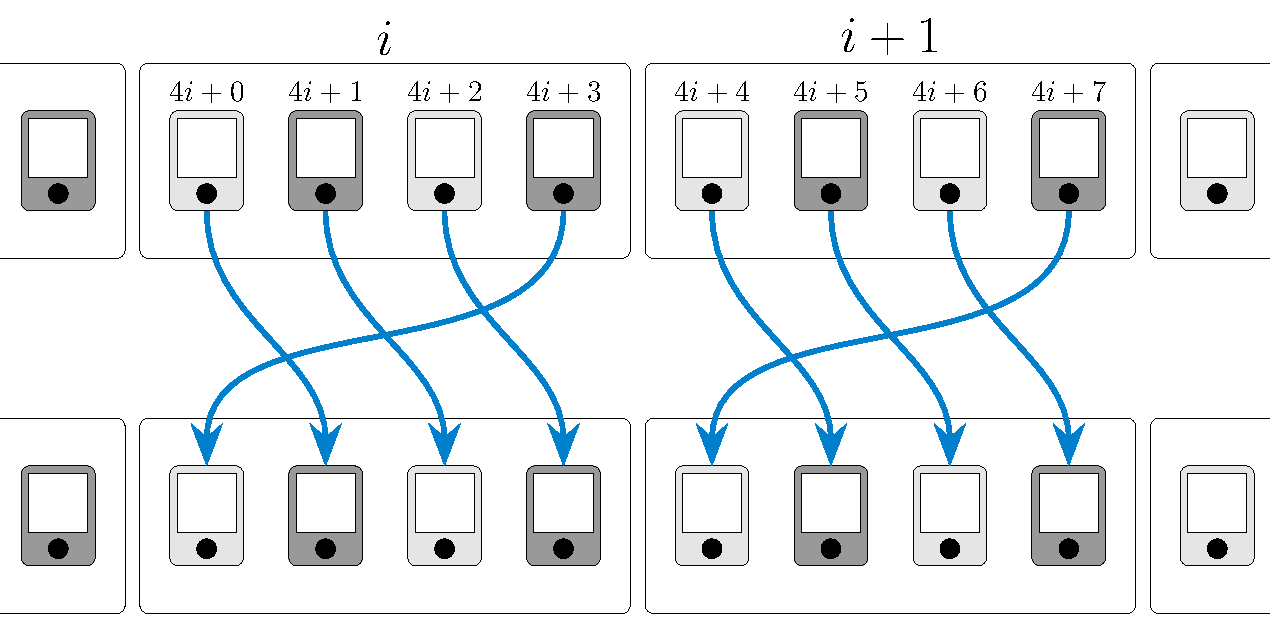
\includegraphics[width=\linewidth]{figures/quad-edge-struct-rot.pdf}
  \end{subfigure}
  \caption[Quad-Edge Rotation Scheme]{
    \textbf{Quad-Edge Rotation Scheme}\\
  }
\end{figure}

% section quad_edge_algebra (end)
\end{document}
